\let\negmedspace\undefined
\let\negthickspace\undefined
\documentclass[journal]{IEEEtran}
\usepackage[a5paper, margin=10mm, onecolumn]{geometry}
%\usepackage{lmodern} % Ensure lmodern is loaded for pdflatex
\usepackage{tfrupee} % Include tfrupee package

\setlength{\headheight}{1cm} % Set the height of the header box
\setlength{\headsep}{0mm}     % Set the distance between the header box and the top of the text

\usepackage{gvv-book}
\usepackage{gvv}
\usepackage{cite}
\usepackage{amsmath,amssymb,amsfonts,amsthm}
\usepackage{algorithmic}
\usepackage{graphicx}
\usepackage{textcomp}
\usepackage{xcolor}
\usepackage{txfonts}
\usepackage{listings}
\usepackage{enumitem}
\usepackage{mathtools}
\usepackage{gensymb}
\usepackage{comment}
\usepackage[breaklinks=true]{hyperref}
\usepackage{tkz-euclide} 
\usepackage{listings}
% \usepackage{gvv}                                        
\def\inputGnumericTable{}                                 
\usepackage[latin1]{inputenc}                                
\usepackage{color}                                            
\usepackage{array}                                            
\usepackage{longtable}                                       
\usepackage{calc}                                             
\usepackage{multirow}                                         
\usepackage{hhline}                                           
\usepackage{ifthen}                                           
\usepackage{lscape}
\begin{document}

\bibliographystyle{IEEEtran}
\vspace{3cm}
\title{11.16.4.7.3}
\author{EE24BTECH11028 - Jadhav Rajesh}
% \maketitle
% \newpage
% \bigskip
{\let\newpage\relax\maketitle}

\renewcommand{\thefigure}{\theenumi}
\renewcommand{\thetable}{\theenumi}
\setlength{\intextsep}{10pt} % Space between text and floats


\numberwithin{equation}{enumi}
\numberwithin{figure}{enumi}
\renewcommand{\thetable}{\theenumi}
 \textbf{QUESTION:} A and B are two events such that $P\brak{A}=0.54$, $P\brak{B}=0.69$ $P\brak{A \cap B}=0.35$. Find $\brak{iii}P\brak{A \cap B'}$\\
\textbf{Theoretical Solution:\\}
\begin{align}
 \brak{A \cap B}=\brak{A\cdot B}
\end{align}\\
For 2 Boolean variables $A$ and $B$, the axioms of Boolean Algebra are defined as:
\begin{align}
    A=AB+AB'
\end{align}\\
\begin{align}
    A\cdot A = A
\end{align}
\begin{align}
    B \cdot B' = 0
\end{align}
Now let's take\\
    $X.Y= AB.AB'=0$,because it is a disjoint\\
 using these axioms, we will try to prove that\\
 \begin{align}
     Pr\brak{A}=Pr\brak{AB}+Pr\brak{AB'}
 \end{align}\\
 \begin{align}
     Pr\brak{A} -Pr\brak{AB} = Pr\brak{AB'}
 \end{align}\\
 Using the given values of $Pr\brak{A}$ , $Pr\brak{B}$ and $Pr\brak{A\cdot B}$\\
 \begin{align}
           Pr\brak{AB'} = Pr\brak{A} -Pr\brak{AB}
 \end{align}\\
 \begin{align}
  Pr\brak{AB'} = 0.54 - 0.35
 \end{align}\\
 \begin{align}
 Pr\brak{AB'} = 0.19
 \end{align}\\
 \textbf{Simulated Solution:\\}
Let $X_1$ be an indicator random variable of the event $A$.\\
$X_1$ is defined as:
\begin{align}
	X_1 =
	\begin{cases}
		1 ,& A\\
		0 ,& A^\prime\\
	\end{cases}
\end{align}
Let $X_2$ be the indicator random variable of the event $B$.\\
$X_2$ is defined as:
\begin{align}
	X_2 =
	\begin{cases}
		1 ,& B\\
		0 ,& B^\prime\\
	\end{cases}
\end{align}
Let $X_3$ be the indicator random variable of the event $AB$.\\
$X_3$ is defined as:
\begin{align}
	X_3 =
	\begin{cases}
		1 ,& AB\\
		0 ,& \brak{AB}^\prime\\
	\end{cases}
\end{align}
The PMF of the random variable $X_1$ is:
\begin{align}
	p_{X_1}\brak{n} =
	\begin{cases}
		p_1 ,& n = 1\\
		1 - p_1 ,& n = 0
	\end{cases}
\end{align}
The PMF of the random variable $X_2$ is:
\begin{align}
	p_{X_2}\brak{n} =
	\begin{cases}
		p_2 ,& n = 1\\
		1 - p_2 ,& n = 0
	\end{cases}
\end{align}
The PMF of the random variable $X_3$ is:
\begin{align}
	p_{X_3}\brak{n} =
	\begin{cases}
		p_3 ,& n = 1\\
		1 - p_3 ,& n = 0
	\end{cases}
\end{align}
where,
\begin{align}
	p_1 &= 0.54\\
	p_2 &= 0.69\\
	p_3 &= 0.35\\
\end{align}
Let $Y$ be the random variable which is defined as follows:
\begin{align}
	Y = X_1 - X_3
\end{align}
\begin{align}
	p_{Y}\brak{n}=
	\begin{cases}
		p ,& n = 1\\
		1 - p ,& n = 0
	\end{cases}
\end{align}\\
Where
\begin{align}
    p = P\brak{A.B'}
\end{align}
Using Expectation to Find $p$:From linearity of expectation
\begin{align}
    E\brak{Y}=E\brak{X_{1}} - E\brak{X_3}
\end{align}
Since
\begin{align}
    E\brak{X_{1}}=p_{1}=0.54,E\brak{X_{3}}=p_{3}=0.35
\end{align}
We have
\begin{align}
    p=E\brak{Y}=p_{1}-p_{3}
\end{align}
Substitute the
\begin{align}
    p=0.54-0.35
\end{align}
\begin{align}
    p=\brak{AB'}=0.19
\end{align}
\begin{figure}[h!]
   \centering
   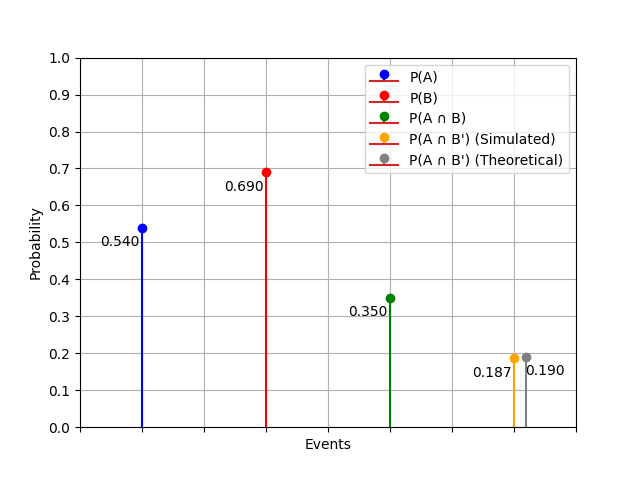
\includegraphics[width=1\columnwidth]{figure/fig.png}
   \caption{Solving the system of equations}
   \label{stemplot}
\end{figure}


 \end{document} 
